\chapter{Temperature, and other species}\label{ch:temperature}

\section{The floor is a function of temperature}

The Mahaffey number falls as body temperature rises, if the free energy of ATP hydrolysis is held fixed: 22.94 for a salmonid
at 10~\textdegree C, 20.94 for a human at 37~\textdegree C, 20.84 for a dog at 38.5~\textdegree C, 20.74 for a bird at
40~\textdegree C. \calc{} Holding $\dGATP$ fixed is an assumption; the free energy depends on temperature and on the cell's
ATP, ADP and phosphate concentrations.

The floor of Eq.~\eqref{eq:eps0} makes a sharper statement. If a cell holds each site with a fixed energy $E_{\rm hold}$,
measured at 37~\textdegree C as $3.41\,\kB T$, then at another temperature
\begin{equation}
  \varepsilon_0(T)=\frac{1}{1+\exp\!\left(E_{\rm hold}/\kB T\right)} ,
  \label{eq:eps0T}
\end{equation}
with no exponent to choose. \derived{} given a fixed holding energy. At 10~\textdegree C this gives $\varepsilon_0=0.0233$ and a
floor $0.78$ times the human one; at 38.5~\textdegree C, $1.012$ times (Figure~\ref{fig:eps0T}). \calc{} The alternative is a
cell that holds its error fixed in units of $\kB T$, adjusting its holding energy with temperature. The two are distinguished by
one measurement.

\begin{figure}[htbp]\centering
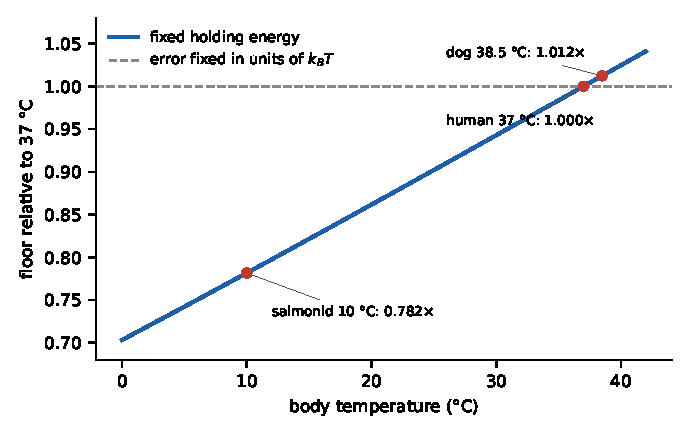
\includegraphics[width=0.8\textwidth]{figures/part4/fig_eps0_T.pdf}
\caption{The floor against body temperature. Solid: fixed holding energy ($3.41\,\kB T$ at 37~\textdegree C), Eq.~\eqref{eq:eps0T}.
Dashed: error held fixed in units of $\kB T$. Marks: dog (38.5~\textdegree C), human (37~\textdegree C), salmonid
(10~\textdegree C). \calc}
\label{fig:eps0T}
\end{figure}

\section{What the fish say so far}

Four salmonid sets have been read with the same single-molecule statistic, three of them pre-registered (Chapter~\ref{ch:salmonid}):
\begin{center}\small
\begin{tabularx}{\linewidth}{@{}>{\raggedright\arraybackslash}X>{\raggedright\arraybackslash}X>{\raggedright\arraybackslash}X>{\raggedright\arraybackslash}X@{}}\toprule
set & tissue, method & holding energy & instrument \\\midrule
Methow River steelhead, 20 fish & red blood cells, RRBS & 3.31 $\kB T$ (median) & halves agree, ICC 0.998 \\
 & sperm, RRBS & 4.02 $\kB T$ & \\
brook charr, 40 males & sperm, WGBS & 3.82 $\kB T$ & ICC 0.92 \\
Rimouski Atlantic salmon, 64 fish & fin, WGBS & 3.47 $\kB T$ (F0) & ICC 0.996 \\
coho smolts, 39 fish & RRBS & 3.30 $\kB T$ & ICC 0.83 \\\bottomrule
\end{tabularx}
\end{center}
\measured{} The instrument repeats almost perfectly in every set. In every set the small differences between fish track the
library (conversion failure, duplicate fraction), so no fish-level difference has yet been read. The steelhead red cells, at
about 10~\textdegree C, read close to healthy human cells at 37~\textdegree C on the same statistic, against the fixed-energy
prediction of a higher value in $\kB T$ units. That comparison is not the test: one small study, reduced-representation
sequencing of CpG-dense regions against whole-genome human reads, a nucleated red cell against human granulocytes, and a
body temperature assumed from the water. \openprob

Figure~\ref{fig:p4_fish} shows every fish on the human statistic and the library terms that the small differences between fish follow.

\begin{figure}[htbp]\centering
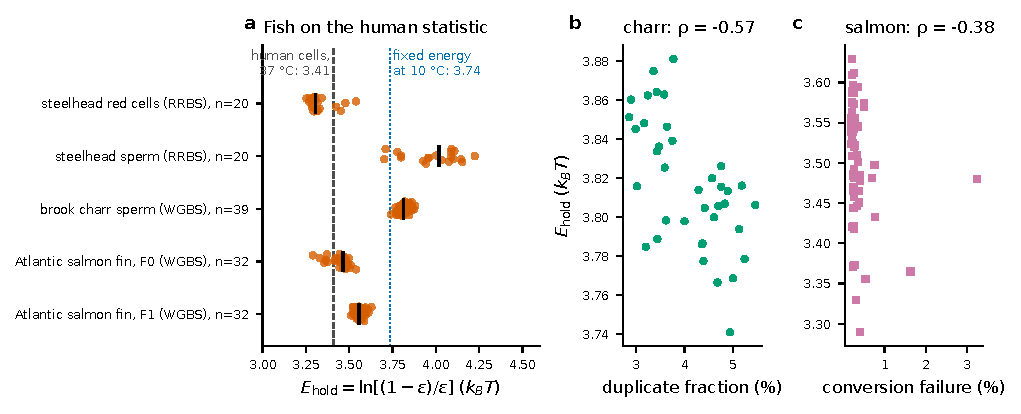
\includegraphics[width=0.98\textwidth]{figures/part4/fig_p4_10_fish.pdf}
\caption{Salmonids on the single-molecule statistic. (a) Holding energy per fish; bar: median (steelhead red cells 3.31, sperm 4.02;
brook charr sperm 3.81, 39 fish with a complete run; Atlantic salmon fin F0 3.47, F1 3.56, in $\kB T$). Dashed: human cells at
37~\textdegree C, 3.41; dotted: a fixed holding energy carried to 10~\textdegree C, 3.74. (b) Charr: holding energy against the library's duplicate
fraction (Spearman $\rho=-0.57$). (c) Salmon: against conversion failure ($\rho=-0.38$; the sign is reversed from that of the copy error).
Data: \texttt{doors/\allowbreak{}data/\allowbreak{}salmon\_readings.csv}, \texttt{charr\_readings.csv}, \texttt{rimouski\_readings.csv}.
\measured{} points; \calc{} dotted line.}
\label{fig:p4_fish}
\end{figure}

\begin{keybox}[title=The test that decides]
One species, one cell type, one read pipeline, at two recorded temperatures. A rearing-temperature experiment does it; a
public whole-genome coho data set (BioProject PRJNA641939), downloaded and not yet read, would give the first fish reading on a pipeline comparable to the human one. Until then
the temperature behaviour of the floor is \openprob, and no ectotherm is read on the gauge.
\end{keybox}

\section{Dogs}

Dogs are the natural first mammal after humans: their blood is drawn routinely, they share our environment, and a
methylation array designed for mammals covers conserved CpGs across species~\cite{Arneson2022}. For a dog $M=20.84$ and the
floor moves by about 1~\%. The first step is a canine healthy reference from purified canine blood cells; then sorted healthy
canine cells read on it, held out, should land at 1.00. \prediction
